\chapter{Marko teorikoa}\label{cha:markoa}
Lan hau kokatzen den marko teorikoa aztertzen hasteko garrantzitsua da hezkuntza teknologikoak egungo hezkuntza sisteman duen rola ulertzea. Horretarako, zer den teknologia jakin behar da lehenik eta behin. Teknologia, \citeauthor{harluxet2019awareness}-k (\citeyear{harluxet2019awareness}, 2. definizioa) egindako definizio entziklopedikoan oinarrituz, gizakiak erabiltzen dituen tresna, makina, prozedura eta metodo teknikoen multzoa. Definizioa kontuan izanda, hezkuntza bera teknologia bat dela ondorioztatu daiteke.

\section{Hezkuntza teknologikoa}\label{sec:heztek}

Hausnarketarekin aurrera jarraituz, bi galdera formulatu daitezke. Lehena, zein da hezkuntzak duen funtzioa gure gizartean? Bigarrena, eta esaldi korapilatsu bat sortuz: hezkuntza teknologia bat izanda, zertarako irakasten da hezkuntza teknologikoa?

Hezkuntzak gizartean duen funtzioaz hitz egiterakoan, gazteria etorkizunerako prestatzea dela esan daiteke. Teknologia bat izanik, prozesu multzo bat da, ikasle bat ume izatetik heldu izan arte igarotzen dena, jakintzak eskuratzen joateko. \citeauthor{tarabini2020que}-k (\citeyear{tarabini2020que}) aipatzen duen bezala, historian zehar, gizarte kapitalista agertu zenetik, korronte desberdinek ondorio berdina izan dute: hezkuntzaren funtzioak bi dira, pertsona lan munduan integratzeko prestatzea eta gizartean integra daitekeen pertsona identitatea sortzea. Beraz, teknologia honen funtzioa zehaztuz, jakintza, ezagutza eta trebakuntzaren transmisioa dela esan daiteke, aurrez aipatu diren bi helburuak lortzeko.

Puntu honetara iritsita, pentsa daiteke hezkuntza teknologikoaz hitz egiten denean, gizartearen historian garatu diren prozesu teknologikoen inguruko ezagutza transmititzeaz hitz egiten dela. Baina hau ez da horrela. \citeauthor{tarabini2020que}ren (\citeyear{tarabini2020que}) testuan irakur daitekeen moduan, sistema kapitalistaren menpe dago hezkuntza, eta XX. mende amaieratik iraultza teknologiko etengabean dagoen sistema da hau (\citeauthor{del2016industria}, \citeyear{del2016industria}; \citeauthor{ghobakhloo2020industry}, \citeyear{ghobakhloo2020industry}). Beraz, kapitalismoaren beharrei erreparatuz, ezin da finkatu hezkuntza teknologikoaren helburua zein izango den datorren urteak ikasten igaroko dituen ikasle batentzat: iraultza aurrera doan heinean, lan mundura integratzeko behar dituen trebetasunak aldatuz joan daitezke, eta zentzugabekeria da uneko trebetasunen jakintza garatzea, urteak aurrera egin ahala zaharkituak geratu daitezke eta. Horregatik, eta \citeauthor{sole2020cambio}-k (\citeyear{sole2020cambio}) aipatzen duen moduan, hezkuntza sistemaren joera konpetentzien garapenera doa. Baina konpetentziekin hasi baino lehen, XXI. mendeko gizartea ulertu behar da.

\subsection{XXI. mendeko gizartearen erronkak}\label{subsec:xxi_erronkak}

Gaur egungo gizarte mailako erronka orokorrak definitu eta horiei aurre egiteko, 2000-2015 milurteko garapeneko helburuak berreskuratuz, 2015eko irailaren 25ean Agenda 2030 onartua izan zen Nazio Batuen asanblada orokorrean. Bertan, Garapen Iraunkorreko Helburuak (GIH) zehazten dira, zeinak politika publikoak hobetu eta lehentasunak definitzeko kontestu bat finkatzen duen lurralde bakoitzeko errealitatea kontuan edukiz (\citeauthor{vasco2017contribucion}, \citeyear{vasco2017contribucion}).

Agenda honen barruan zehazten diren edukietan sakonduz, garapen iraunkorrerako 17 helburu zehazten dira. Helburu hauek, ekintzarako dei unibertsal bat dira pobreziarekin amaitzeko, planeta babesteko eta mundu osoko pertsonen bizitza eta aukerak hobetzeko (\citeauthor{nbe2021}, \citeyear{nbe2021}). Hauek guztiak, planetarentzat eta gizartearentzat orokorrean garrantzia berezia duten 5 esfera landuz burutu nahi dira.

\begin{itemize}
    \item Pertsonak: pobrezia eta gosea amaitzea bere forma eta dimentsio guztietan, eta pertsona guztiek beraien ahalmenak duintasunez, berdintasunean oinarrituta eta ingurune osasuntsu batean bete dezaketela bermatzea.
    \item Planeta: degradaziotik babestea kontsumo eta ekoizpen jasangarrien, baliabide naturalen kudeaketa jasangarriaren eta aldaketa klimatikoari aurre egiteko neurri zehatzen bidez. Modu honetan, gaur egungo eta etorkizuneko belaunaldien beharrei erantzunez.
    \item Bakea: indarkeria eta beldurrik gabeko gizarte baketsu, justu eta inklusiboak sustatzea.
    \item Oparotasuna: pertsona guztiek bizitza oparo bat izan dezatela ziurtatzea eta garapen ekonomiko, sozial eta teknologikoa naturarekin bat etorriko dela ziurtatzea.
    \item Lankidetza: agenda ezartzeko beharrezkoak diren bitartekoak martxan jartzea mundu mailako aliantza baten bitartez garapen iraunkorra inplementatzeko. Guzti hau, mundu mailako elkartasun handiago batean oinarrituta eta bereziki pobreenen eta ahulenen beharretan arreta jarriz. Baina hau herrialde guztietako eragile eta pertsonen lankidetzarekin gauzatuta.
\end{itemize}

EAEn hau guztia lurreratzeko, I. Agenda Euskadi Basque Country 2030 dago, zeina 17 helbururen inguruan egituratzen den. Helburu hauek, herrialdeko 15 helburuei lotuta daude eta guztira 100 meta definitzen dira (\citeauthor{vasco2017contribucion}, \citeyear{vasco2017contribucion}).

Hezkuntza komunitateak ere aipaturiko norabidea elikatzeko konpromisoak hartuak ditu. Horren adibide da, Eskola Agenda 2030 programaren existentzia eta sortu zenetik, bataz beste, urtero 450 ikastetxe (publiko, itunpeko zein pribatu), 200.000 ikasle baino gehiago eta 15.000 irakaslek bertan parte hartu izana (\citeauthor{dv2021}, \citeyear{dv2021}). Horrez gain, aurrerago zehaztuko den moduan, hezkuntza teknologikoaren helburua eta dinamika bera, erabat bideratuta daude gizarte moduan ditugun erronka eta beharrei erantzun egoki bat ematera. Beraz, ezinbestekoa da lehenik eta behin egungo egoeraren analisi kritiko bat egitea eta jarraian, horiei erantzungo dieten planteamenduak garatzea. 

Erronka hauen baitan, hezkuntza mugimendu bat du da azken urteetan. Arazo garaikideei aurre egiteko hezkuntza digitalean burujabetza eta pentsamendu kritikoa nabarmentzea nahi dituena.

\subsection{Zientzia, Teknologia eta Gizartea}\label{subsec:ztg}

Alde batetik, gaur egungo gizartea etengabeko berrikuntza eta aldaketek ezaugarritzen dute. Hori dela eta, baliabide materialen (azpiegitura, makinak) beharrezkotasuna bigarren planoa batean geratzen da, geldiezinak diren berrikuntzen ondorioz azkar batean zaharkituta geratzen direlako. Kontestu honetan, baliotsuena norbanakoek sormenez, arduraz eta kritikoki ezagutzak sortu, elkarbanatu eta aplikatzeko duten gaitasunak dira (\citeauthor{acevedo1998ciencia}, \citeyear{acevedo1998ciencia}). 

Beste alde batetik, ezin uka daiteke teknologiak hartu duen garrantzia bizitzako alor guztietan eta hori dela eta, honen aldeko, kontrako edo erdi bideko posizioak hartuz joan dira hainbat esparru, \citeauthor{acevedo1998ciencia}ren (\citeyear{acevedo1998ciencia}) testuan irakurri daitekeen bezala. Teknologiarekiko jarrera ezberdin hauen arrazoi nagusia honek gizartean izan duen eraginean datza.

Nahiz eta teknologiak hainbat hobekuntza nabarmen ekarri herritarrei, honek aberatsen eta pobreen arteko arrakala handitzea ekarri du. Hau da, herrialde, lurralde eta talde sozial aberatsak geroz eta aberatsago izatea eta pobreak geroz eta pobreago izatea, nahiz eta, hasiera batean kontrakoa uste zen (\citeauthor{osorio2002educacion}, \citeyear{osorio2002educacion}).

Horren adibide da, Munduko Bankuaren datuen arabera, 2012an 896 milioi pertsonak eguneko 1,9\$ baino gutxiagorekin biziraun izana (\citeauthor{migoyaxxi}, \citeyear{migoyaxxi}). \citeauthor{menendez2017europe}-k (\citeyear{menendez2017europe}) egindako txostenak adierazten du pobrezia profil berri bat sortu dela. Pobrezian bizi diren pertsona hauek lan egiten duten (lanaldi partzialak, aldi baterako kontratuak edo lan autonomoak) baina aldi berean pobreak dira. Gaur egun, Europako langileen \%10ek osatzen dute profil hau.

Kontestu konplexu honetan, zientzia eta teknologiak soilik paper bat jotzen du gaur egungo joko zelaian eta jakinekoa da teknologia eta zientziak beste orientazio sentikorrago bat hartzen ez badute, aipatutako egoerak okertzen lagunduko dutela soilik dio \citeauthor{osorio2002educacion}k (\citeyear{osorio2002educacion}). Hori dela eta, ezinbestekoa da hezkuntza aktore klabe moduan hartuz, bertatik zer egin daitekeen aztertu eta garatzea.

Hezkuntzak funtzio sozial garrantzitsuak betetzen ditu. Tartean, berriz ere \citeauthor{acevedo1998ciencia}ren (\citeyear{acevedo1998ciencia}) hitzez baliatuz, belaunaldi berriei gizarte produktibo batean behar bezala funtzionatzeko gaitasun ezberdinak eskaintzea, nahiz eta etengabeko aldaketen ondorioz, hezkuntzaren funtzioa gizarteko partaide guztiengana luzatu, bizi osorako ikaskuntza ardatz hartuz.

Orain arte aipatu moduan, teknologia eta zientziak bizitzako esparru guztietan duen garrantziagatik eta belaunaldi berriak etorkizuneko erronkei aurre egiteko prest egoteko, hezkuntza teknologiakoren beharra ezinbestekoa da.

Hezkuntza teknologikoa, teknikak ulertu, hautatu, erabili, egokitu, ebaluatu eta sortzeko eta, azken finean, teknologiak ekoizteko aukera ematen dion prestakuntza da. Hau da, bakoitzaren ingurune teknologikoa modu naturalean arakatzen laguntzea eta kontsumitzaile kritiko eta erabiltzaile adimenduna izatea (\citeauthor{grau2016educacion}, \citeyear{grau2016educacion}).

Honen bitartez, hezkuntza ingurune teknologiko eta zientifikora zabaltzeko aukera eskaintzen da, horren gainean modu arrazionalean jarduteko. Horrez gain, ezagutzak batu eta horiek prozesu didaktiko bakarrean biltzea eta aldi berean, lanerako eta goi mailako ikasketetarako prestatzea. Azkenik, \citeauthor{grau2016educacion}k (\citeyear{grau2016educacion}) dioen moduan, ikasleen orientazio profesionalaren lagungarri izateko aukera ere ematen du.

Laburbilduz, hezkuntza teknologikoaren kontzeptua globala da eta inplikazio gradu, maila eta modalitate ezberdinak inplikatzen ditu, zeren eta bere helburua ez da ikaslea teknologikoa edo teknologian espezializatua izatea. Azken finean, hezkuntza teknologikoaren bidez balioetan oinarritutako hezkuntza txertatzea da xedea, hau da, teknologiak baloratzeko eta hauen ondorioak ebaluatzeko heztea, teknologien ebaluazioan publikoaren parte- hartzea ahalbidetzeko ezinbestekoa dena (\citeauthor{martin2000acercando}, \citeyear{martin2000acercando}).

Kontestu honetan, garrantzitsua da teknologiaren erabilera sustatzea ikuspegi humanista, kritiko eta arduratsu batetik, ikasleek ezagutzak sortu, ideiak transmititu, irtenbideak identifikatu eta produktu zehatzak garatzeko norberaren interesen arabera (\citeauthor{leal2019}, \citeyear{leal2019}).

Nahiz eta teknologia oso presente eduki egunerokotasunean, sarritan honen ikaskuntza termino abstraktuetan geratzen da. Horregatik, ikasleak teknologiaren baliagarritasunaz ohartarazteko garrantzitsua da hainbat gako kontuan edukitzea.

Alde batetik, teknologia proiektuak garatzeko erreminta bezala ulertzea. Hau da, ikasleen eskura egongo den erreminta bezala ulertzea teknologia eta ez alderantziz. Horretarako, \citeauthor{leal2019}en (\citeyear{leal2019}) ustetan, interesgarria ikusten da lantzen ari diren materiak teknologiako proiektu espezifikoekin lotzea. Beste alde batetik, garrantzitsua da tresna digitalen erabilera beste ikasgai batzuetara zabaltzea, beste ikasgai horien ikaskuntza bultzatu eta errazteko. Horretarako, beharrezkoa da alde batetik irakasleen mesedetara baliabide digitalak jartzea baina bereziki irakasleek ikasleak kontzientziatzea baliabide hauen erabilerak beraien ikaskuntza prozesua hobetuko duela.

Horrez gain, teknologiak sormena garatzeko, konponbideak sortzeko eta arazoak konpontzeko gaitasuna du. Horregatik, ikasleek beraien ikaskuntza prozesuak sinplifikatzeko, irtenbide sortzaileak sortzeko, proposamenak egiteko eta ideiak adierazteko teknologia bultzatu nahi da.

\citeauthor{leal2019}en (\citeyear{leal2019}) teoriarekin jarraituz, zientzia eta teknologiak aldaketa sakonak eragin dituzte alor sozial, ekonomiko, teknologiko eta mediatikoan. Horregatik, ikasleek horrekiko ikuspuntu kritiko bat garatzea garrantzitsua ikusten da hezkuntzako idealen parte delako eta aldi berean, ikasleek proposamenak egiteko erabiltzea ikuspegi humanista bultzatu eta aldaketa soziala bultzatuz.

Honetaz guztiaz gain, teknologiaren erabilera seguru eta arduratsua irakastea ikasleei. Elkarrekintzarako forma berriak erabiltzen diren momentutik, arrisku eta gatazka etiko berriei aurre egin behar zaie. Horregatik, garrantzitsua da teknologiaren erabilera arduratsu eta etiko bat bultzatzea. 

Hezkuntzako hainbat sektoretatik, ikasleei informazio eta ezagutza baino, eguneroko bizitzari aurre egiteko gaitasunak emateko beharraz ari dira. Horien artean egongo lirateke, talde lanarekin, komunikaziorako trebetasunekin, arazoen ebazpenarekin eta erabakiak hartzearekin lotutakoak. Horrez gain, mundu ikuskera zientifiko eta teknologiko bat duten ikasleak trebatzea espero du \citeauthor{acevedo1998ciencia}k (\citeyear{acevedo1998ciencia}). Aldi berean, hezkuntza teknologikoaren kontzepziotik, honek aukera handiak eskaintzen ditu konpetentzietara, disziplinartekotasunera, ikasleen motibaziora, gaien egokitasunera hurbiltzeko.

Orain arte aipatutako aspektu eta ezaugarri guztiak kontuan hartu eta bide horretan ekarpena egiten du Zientzia, Teknologia eta Gizartea (ZTG siglekin adierazia) mugimenduak.

Termino honek barne- biltzen dituen hiru aspektu nagusietan sakonduz, jakitun gara zientzien eta teknologiaren arteko bereizketa kritiko bihurtu dela, lehena alderdi askotan bigarrenaren zerbitzura dagoelako. Zentzu horretan, “tekno- zientzia” terminoak zientzia eta teknologiaren arteko hurbilpen bat gauzatzen du, politika, ekonomia eta ingurugiroarekin batera. Aldi berean, ZTG mugimenduak, zientzia eta teknologiaren garapena ingurune sozial eta politiko batean kokatzen ditu (\citeauthor{osorio2002educacion}, \citeyear{osorio2002educacion}).

Mugimendu honen helburua herritarren alfabetatze zientifiko eta teknologikoa sustatzea da, erabakiak hartzeko prozesu demokratikoetan eta zientzia eta teknologiarekin lotutako arazoen ebazpenetan parte har dezaten (\citeauthor{membiela1997revision}, \citeyear{membiela1997revision}).

Aipatutako lan egiteko proposamen hau zehaztuz, \citeauthor{hickman1987science}-ek (\citeyear{hickman1987science}) kontuan eduki behareko bost kriterio nagusi zehazten zituzten ZTG- ko edukietan:

\begin{itemize}
    \item Ea zuzenean aplikatu daitezkeen lantzen diren edukiak ikasleen eguneroko bizitzetan.
    \item Ea edukiak egokiak diren ikasleen garapen kognitibo eta heldutasun sozial mailarako.
    \item Lantzen ari den gaia gaur egun munduan ikasleentzat eta aldi berean helduentzat garrantzitsua ote den.
    \item Ezagutza horiek eskolaz kanpoko testuinguruetan aplikatu daitezkeen.
    \item Ikasleek interesa, ilusioa eta lanerako gogoa erakusten duten gaia ote den.
\end{itemize}

ZTGekiko lotura duten arazo sozialen arabera, 2 perspektiba nagusi definitzen ditu \citeauthor{rosenthal1989two}-ek (\citeyear{rosenthal1989two}). Alde batetik, komunitate zientifikotik kanpoko gizarte- gaiak, hala nola, berotze globala, gerra kimikoa edo elikagaietako pestizidak. Bestetik, komunitate zientifikoaren barneko gizarte- gaiak, zientziaren gizarte- ikasketa moduan deitzen direnak, non zientzia bera den gizarte- zientzien aztergai bere ondorio filosofiko, soziologiko, historiko, politiko, ekonomiko eta kulturalak jorratuz.

Mugimendu honen printzipioak eta edukiek izan beharreko ezaugarriak definitu ondoren, hau guztia ikasgelara nola lurreratu zehaztea beharrezkoa da. Nahiz eta unibertsitate eta bigarren hezkuntzako eremuetan garatu den mugimendu honen jarduna (\citeauthor{membiela1997revision}, \citeyear{membiela1997revision}), bigarren hezkuntzan ZTG markoaren printzipioak nola lurreratzen diren lantzen da. Horretarako hiru modu edo bide nagusi daude.

Horietako bat, ZTG txertoak izango litzateke. Ikasleak zientziaren eta teknologiaren ondorioez jabetzera bultzatzen dituzten alderdiekin lotutako arazoetarako tresna garrantzitsua bihurtzen dira (\citeauthor{osorio2002educacion}, \citeyear{osorio2002educacion}). 

Konkretuki, zientzia ikasgai bati ZTG alorreko gehikuntza bat egitean datza, beti ere zientziaren izaera eta teknologiarekin eta gizartearekin dituen inplikazioak berrikusi beharko lituzkeena. Baita ere aldi berean, herritarrek duten papera garapen tekno- zientifikoaren inguruko erabakietan.

Teknologiako ikasgai batean berriz, ZTG ikuspegian gehiago sakondu beharko litzateke, teknologiaren izaeraren, teknologiaren eta gizartearen arteko harremanen eta teknologiaren eta zientzien arteko ikuspegitik (\citeauthor{osorio2002educacion}, \citeyear{osorio2002educacion}).

Beste bat berriz, zientzia eta teknologia ZTGen bitartez izango litzateke. Zientzia gaietan arazoak dituzten ikasleek kontzeptu zientifiko eta teknologiko erabilgarriak ikasten dituzte ikastaro mota hauetatik, edukiek ikasleen eskolaz kanpoko esperientziekin lotura dutelako. Honen adibide praktiko bat, Holandan jarritako proiektu bat izango litzateke. Unitate bakoitzean ikaslearen etorkizuneko eginkizunekin lotutako oinarrizko arazo bat hartzen da. Hortik aurrera, beharrezko ezagutza zientifiko eta teknologikoa aukeratzen eta egituratzen da, ikaslea erabakiak hartu eta gai sozial batekiko ikuspuntu bat ulertzeko gai izan dadin (\citeauthor{gonzalez1996ciencia}, \citeyear{gonzalez1996ciencia}).

Hirugarren modua ZTG \textit{pura} moduan izendatzen da. Modu honi lotutako adibide esanguratsu bat Asturiasen martxan jarritako \textit{Proyecto Argo} izango litzateke. Hiru ataletan banatzen da proiektua: Lehenengoan, zientzia, teknologia, gizartea, eta ZTG ikasketak kontzeptualizatzen dira. Bigarren, atalean, zientzia, teknologia eta gizarteak izan dituen harreman historikoak lantzen dira eta hirugarrenean, erabaki tekno-zientifikoen ebaluazioaren eta gizarte- kontrolaren gaian zentratzen da (\citeauthor{osorio2002educacion}, \citeyear{osorio2002educacion}).

\subsection{ZTG + I}\label{subsec:ztgi}

Gaur egungo gizartearen bilakaerarekin batera, ZTG mugimenduaren ikuspegia ere aldatzen doa beste hainbat aspektu horren baitan txertatuz. Horren adibide da ZTG + I tendentzia, hau da, ZTG ikuspegiari ingeniaritza ikasketak txertatzea. Modu horretan Industria 4.0k eskatzen dituen ondo formatutako teknikoen beharrari erantzunez eta horrez gain, formakuntzarako espazio eta materialak eskainiz gazteak hiritartasun tekno-digitaleko hezkuntza jasotzeko (\citeauthor{toscano2017}, \citeyear{toscano2017}).

Azken finean, ingeniarien profesioa da zientzia eta teknologiarekin lotutako lanbideetatik ingurunearen baldintzak aldatzeko eta gizakiaren eta ingurunearen arteko interfazeak eraikitzeko gaitasun handiena duena. Eginkizun horretan, ingeniari modernoak dimentsio politiko, ekonomiko, soziologiko, ingurumen, psikologiko eta etikoetan eragin behar du (\citeauthor{toscano2017}, \citeyear{toscano2017}).

Laburbilduz, ZTG + I joera 4 helburu nagusirekin jardun nahi du:
\begin{itemize}
    \item Ingeniarien formakuntzan ZTG ikuspegia txertatzea.
    \item Industria 4.0ko gaien inguruan teknikoa presatzea.
    \item Hirugarren adinekoen alfabetatze digitala gauzatzea.
    \item Hiritarrek hezkuntza teknologiko edo digitala jasotzea.
\end{itemize}

\subsection{Konpetentzietan oinarritutako hezkuntza}\label{subsec:konp}

Aurrez aipatu den bezala, XXI. mendeko gizartearen erronkak gainditu ahal izateko, hezkuntza curriculum\footnote{Maila bakoitzeko ikaskuntza prozesua erregulatzen duen prozesuen multzoa.}ak hainbat aldaketa izan ditu, konpetentzietan zentratuz joateko. 1990ean argitaratu zen LOSGE legetik gaur egun indarrean dagoen LOMLOE legerarte (eta dokumentu hau idatzia izaten ari den unean, beste lege baten proposamena martxan dela jakinda), bipartidismoaren ondorio direnaren falazian erortzea erraza da. Aurrez azaldu diren gaiekin lotuko da jarraian. Horretarako, berriz ere \citeauthor{sole2020cambio}ren (\citeyear{sole2020cambio}) kritikaz baliatuz, hezkuntza mundu ekonomikoaren mesedetan eraldatzen doan sistema dela eutsiko da. Sistema ekonomikoarekiko dependentzia honek beharrak betetzeko, hezkuntza moldatu joan da, gaur egun dagoen modelora iritsi arte.

Markoaren hasieran azaldu den kontzeptu bat berreskuratuz, Ekonomiaren motorra, industria, etengabeko iraultzan dago XX. mende amaieratik. Hau dela eta, ezinezkoa da jakitea zein izango den etorkizunean behar izango den jakintza. Horregatik, eta heziketa prozesuan dabilen gazte batek garatu beharreko jakintzen inguruan eztabaidatzean, ezin daitezke finkatu ikasleak etorkizunean jakin beharko dituen eduki zehatzak. Helburuak aztertuz, bigarren hezkuntza burutzean gazte bat bi gauza egiteko gai izan behar da. Lehenengo helburua langileria masara batzea izango da, industriaren behar nagusia asetzeko. Honetarako, bi bide jarraitu daitezke, ikasketa espezializatuak burutzea, arlo zehatz bateko jakintza sakonagoak garatzeko; edo lan munduan berehala integratzea, egungo egoeran zaila den zerbait (\citeauthor{fernandez2016adquisicion}, \citeyear{fernandez2016adquisicion}). Bigarren helburua gizartean integratzea da, eta hau burutzeko ezinbestekoa da lehen helburua betetzea.

Ondorioz, gazte batek bi aukera ditu, lan mundura integratu edo ikasketa nagusiak burutu. Bi hauek izanda jarraituko dituen bideak, eta aurrez aipatutako egoera kontuan hartuta, \citeauthor{ocde2005deseco}\footnote{Euskaraz, Ekonomia Lankidetza eta Garapenerako Antolakundea. Ingelesez \textit{Organization for Economic Cooperation \& Development}.} (\citeyear{ocde2005deseco}) garatutako txostenean hurrengoa ondorioztatzen da: gaur egungo gizarteak, norbanakoak diziplina anitzetako arazoei aurre egitera behartzen ditu. Honela, jakintza finko bat garatu beharrean, konpetentzia malguago bati ematen dio garrantzia. Konpetentzia bat, ELGAren definizioan oinarrituta, trebetasun, jakintza, jokamolde eta balore multzo finko bat da. Konpetentzia bat garatu dela ez da zerbait ikasiz justifikatzen, konpetentzia baten garapena ekintza baten buruketari lotua dago. Hau dela eta, Europar Erkidegoko Batzordea 2006tik hezkuntza curriculumetan konpetentziak integratzen joan da. Hau erantzun logikoa da azken finean, gizartearen beharrei erantzuna da eta (\citeauthor{valle2013competencias}, \citeyear{valle2013competencias}). Joera honekin jarraituz, EAEko kasua aztertuko dugu.

\subsection{EAEko konpetentzien markoa}\label{subsec:eaekomp}

Europar proposamenak jarraituz, eta Espainiako 126/2014 errege dekretua betetzeko, Eusko Jaurlaritzak argitaratutako curriculumean biltzen dira oinarrizko konpetentziak. Sailkapenari begira, bi multzotan daude banatuta konpetentzia hauek: oinarrizko zehar konpetentziak eta oinarrizko diziplina barneko konpetentziak.

\newpage
\begin{center}
    \captionof{figure}{\textit{Oinarrizko zehar konpetentziak}}
    \label{fig:zehar_konpe}
    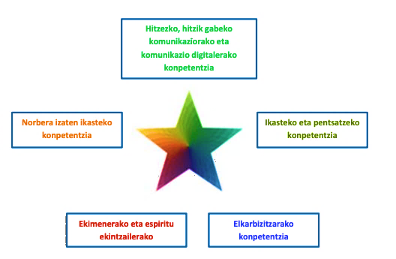
\includegraphics{zehar_konpe}
    \centering
    \par{Iturria: \citeauthor{ej2016curriculuma} (\citeyear{ej2016curriculuma})}
\end{center}

\ref{fig:zehar_konpe} irudian azaltzen den moduan, bost oinarrizko zehar konpetentzia daude dekretatuta. Zehar konpetentzia hauetatik, marko honetarako garrantzitsua dena hau da: hitzezko, hitzik gabeko komunikaziorako eta komunikazio digitalerako konpetentzia. Konpetentzia honen baitan biltzen diren helburuen artean, informazioaren eta komunikazioaren teknologiak modu sortzaile, kritiko, eraginkor eta seguruan erabiltzea dago bilduta, edo beste modu batera esanda, konpetentzia digitala (edo KD, laburtzeko) garatzea. Lan honen gai nagusia hau izanik, nahiz eta gaia ikuspuntu teknologiko batetik jorratu gaia, zeharkako konpetentzia bat izanik hezkuntza osoari eragiten dion zerbait dela ulertu behar da.

Bestalde, eta diziplina barneko konpetentzietan erreparatuz, teknologiarako konpetentzia da testu honekin jarraitzeko ulertu beharrezkoa. Esan den bezala, konpetentzia teknologikoa ingeniaritzan eta industrian erabiltzen diren prozesu eta metodologietan oinarritzen da, baina KDekin oso erlazionatua dagoen atal bat ere badauka konpetentzia honek: informazioaren eta komunikazioaren teknologiak (edo IKTak, laburtzeko). IKTak egungo gizarteko esparru orotan erabiltzen den teknologia da (\citeauthor{graells2000tic}, \citeyear{graells2000tic}). Teknologia hauek, sistema globalizatu batean aurkitzen direnez, multinazionalek garatzen dituzte, eta beraien etekina handitzeko daude garatuak.

Konpetentzia teknologikoa lantzerako orduan, hau da \citeauthor{ej2016curriculuma}k (\citeyear{ej2016curriculuma}) argitaratutako curriculum\footnote{}-ean azaltzen dena:

\begin{adjustwidth}{3em}{0pt}
“Produktu eta sistema teknologikoak zentzuz erabiltzea eta garatzea, jakintza teknikoak eta gainerako adarretako jakintzak era metodiko eta eraginkorrean aplikatuta, interesa duten egoerak ulertzeko eta konpontzeko edota produktu eta zerbitzu berriak eskaintzeko, eta lortutako emaitzen berri ematea, hobekuntza-prozesuekin eta erabakiak modu arduratsuan hartzeko prozesuekin jarraitzeko.”
\end{adjustwidth}

Honekin adierazi nahi dena da, hezkuntza teknologikoko prozesu eta jakintzak bigarren planora mugituz, jakintzaren erabilera kritikoan zentratzen dela konpetentzia garatzean landu nahi dena. Teknologiak gaur egungo gizartean duen pisuaz hitz egingo da, zergatia ulertzeko.

Kontzeptu honekin hasteko, ZTG mugimenduak lantzen dituen ideia nagusiak ulertzeak lagundu dezake. Mugimendu honek duen oinarria teknologiak gizartean duen eragina azpimarratzea da. Mundu globalizatu honetan, gizarteak teknologiarekiko duen dependentzia geroz eta handiagoa dela dirudi, \citeauthor{osorio2002educacion} (\citeyear{osorio2002educacion}) testuetan irakurri daitekeen bezala. Globaletik arlo lokalera itzuliz, dependentzia teknologiko hauen inguruko onurak eta kalteak bereizten jakitea garrantzitsua da, eta ikuspegi kritikoa landu behar da. XXI. mendeko euskal gizarte modernoak dituen erronken erroan aurki daiteke teknologia, zeharka baldin bada ere. Modu batera edo bestera, arlo teknologikoa inplikatuta dago erronka hauetan. Lehen hezkuntzatik datorren gazteak etorkizunean gizarteko erronketan inplikatuta egongo denez, ikuspuntu teknologikoa eta iritzi kritikoa garatzea beharrezkoa da.

Gazteek hezkuntza teknologikoa jasotzen hasi zirenetik, betidanik aipatu da teknologiaren ikaskuntza nola burutu behar den. Nahiz eta teknologia ikasgai bezala irakatsi, hastapenetatik argi izan den gauza da teknologia zeharka eragiten duen ikasgaia dela (\citeauthor{gilbert1995educacion}, \citeyear{gilbert1995educacion}). Azken finean, ezagutza zientifikoari oso lotuta dagoen gaia da, elkarbizitza ohikoa izanez, beraz garrantzitsua da ikasleengan lotura hauen ebidentzia adieraztea. Bestalde, aurrerapen teknologikoak hezkuntzan ere aplikatzen dira, eta aro digital berri baten aurrean aurkitzen da sistema. Eta hau, curriculumaren konpetentzia izaerarekin lotuz, islatuta geratzen da KDen garapenean zentratzen den atalean. Baina honekin jarraitzeko, beharrezkoa da XXI. mendeko euskal gizartearen erronkak ulertzea, eta nola islatzen den hau hezkuntza curriculumean.

Beraz, esparru bereko curriculumeko bi konpetentzia aztertu dira, eta konpetentzia hauetan iritzi kritikoa, neutraltasuna zein burujabetasuna aipatzen dira, baina edukiei begira horrelako lanketarik egiteko emaitzarik ez dagoela ikusten da. Hau honela izanda, bestelako markoetan aurkitu behar izaten da sakontzeko aukera. Jarraian aipatuko den hezitzaileen konpetentzia digitalerako Europar markoak\footnote{Ingelesez, \textit{European Framework for the Digital Competence of Educators}.} (edo DigCompEdu markoa) zerbait gehiago sakontzen du honen inguruan.

\section{Digitalizazioa}\label{sec:digitalizazioa}

Prozesu hau aurreko mendetik datorren joera bat da. Gizarteko alor guztietan aurki daitezke prozesu honen adierazleak, baina hasteko hezkuntzak jaso duen prozesua aztertuko da.

\subsection{DigCompEdu}\label{subsec:digcompedu}

Marko honek Europako hezitzaileen gaitasun digitala garatzeko esparru bat aurkezten du. Helburua, Estatu kideei laguntzea da beren herritarren gaitasun digitala sustatzeko eta hezkuntzaren berrikuntza bultzatzeko ahaleginetan. Markoak hezitzaileen gaitasun digitala sustatzeko, bai nazio, eskualde eta tokiko mailan egiten diren ahaleginak laguntzea du helburu, horretarako, erreferentzia-esparru komun bat eskainiz, hizkuntza eta logika partekatu batekin (\citeauthor{JRC107466}, \citeyear{JRC107466}).

Markoak Europar Batzordeko \textit{Joint Research Centre}-k (JRC) gauzatutako lanean du oinarria, hezkuntza, gazteria, kirol eta kultura Zuzendaritza Nagusiaren izenean.

DigCompEdu markoak Europako kide diren estatuetako kezkari erantzuten dio, hezitzaileen kezka propio bati, hain zuzen. Lanbide honen gaitasun digital multzo baten beharra argi manifestatzen da, teknologia digitalek duten ahalmena aprobetxatu ahal izateko. Honela, hezkuntzan hobekuntzak eta berrikuntzak gauzatuko dira.

DigCompEdu markoaren helburua da hezitzaileen gaitasun digitalerako dauden tresnei buruz hausnartzea eta hezkuntza-maila guztietako hezitzaileei beren gaitasun digital pedagogikoa ebaluatu eta garatzea ahalbidetzen dien eredu koherente batean sintetizatzea.

Hortaz, DigCompEdu-k ondorengo puntuetan azaltzen diren balore erantsiak eskaintzen ditu:

\begin{itemize}
    \item Maila guztietan hezkuntza-politikak bideratu ditzakeen oinarri sendo bat.
    \item Interesa ageri duten tokiko eragileei, beren beharrei egokituta dagoen tresna zehatz bat berehala garatzeko eredua, lan honetarako oinarri kontzeptual bat garatzeko beharrik gabe.
    \item Herrialdeen arteko praktika hoberenak trukatzen eta eztabaidatzen lagungarria izan daitekeen hizkera eta logika bateratu bat.
    \item Estatu kide, beste interes-talde eta beste edozein parte-hartzaileentzako erreferentzia-puntua, beren tresna eta esparruen osotasuna eta ikuspegia baliozkotzeko, bai oraingoak eta bai etorkizunekoak.
\end{itemize}

5.Irudian ikus daitekeen moduan, DigCompEdu markoak sei arlo ezberdin bereizten ditu, hezitzaileen gaitasun digitala nabarmentzen dituen hogeita bi konpetentziarekin osatuta.

\begin{center}
    \captionof{figure}{\textit{DigCompEdu arloak eta irismena}}
    \label{fig:digcompedu_arloak}
    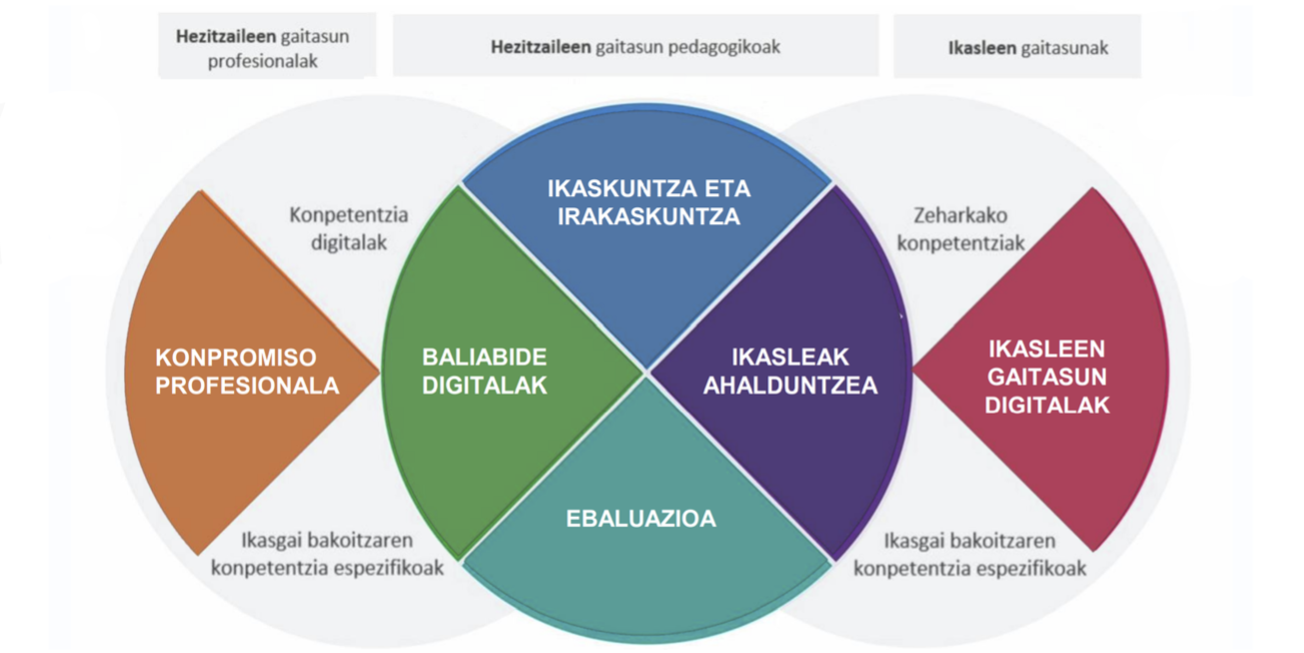
\includegraphics{digcompedu_arloak}
    \centering
    \par{Iturria: Sorkuntza propioa. Abiapuntua: \citeauthor{JRC107466} (\citeyear{JRC107466})}
\end{center}

\citeauthor{JRC107466}en \citeyear{JRC107466} testuan irakurri daitekeenez, irakasleek, gizarteko beste edozein pertsona bezala, gaitasun digitalak behar dituzte. Behar hau, gainera, garrantzitsuagoa da, ondorengo argumentuagatik:

\begin{adjustwidth}{3em}{0pt}
“Irakasleak eredu dira hurrengo belaunaldientzat. Hortaz, behar-beharrezkoa da gizarte digital batean aktiboki parte hartzeko herritar guztiek behar duten gaitasun digitala izatea irakasleek. Edonola ere, irakasleak ez dira ereduak soilik. Oroz gain, ikaskuntzaren gidari dira, edo, are sinplekiago, irakasle. Ikaskuntzan diharduten profesional gisa, ezinbestekoa da, bizitzarako eta lanerako beharrezkoak diren gaitasun digitalez gain, irakasleentzat espezifikoak diren gaitasun digitalak izatea, teknologia digitalak eraginkortasunez erabili ahal izateko irakasteko orduan. DigCompEdu esparruaren helburua irakasleentzat espezifikoak diren gaitasun digital horiek zehaztu eta deskribatzea da.”
\end{adjustwidth}

Beraz, hurrengo zerrendan bilduta daude marko honek biltzen dituen gaitasun digitalen zerrenda, 6 arlotan banatuta.

\begin{enumerate}
    \item arloa. Konpromiso profesionala: garapen profesionalerako, elkarlanean aritzeko eta komunikatzeko teknologia digitalak erabiltzea.
    \item arloa. Baliabide digitalak: eduki digitalak eskuratu, sortu eta partekatzea.
    \item arloa. Irakaskuntza eta ikaskuntza: irakaskuntzan eta ikaskuntzan teknologia digitalen erabileraren kudeaketa eta antolaketa.
    \item arloa. Ebaluazioa eta feedback-a: ebaluazioa hobetzeko teknologia eta estrategia digitalak erabiltzea.
    \item arloa. Ikasleak ahalduntzea: teknologia digitalen erabilera ikaslearen ikaskuntza propioaren baitan inklusioa, pertsonalizazioa eta konpromiso aktiboa areagotzeko.
    \item arloa. Ikaslearen gaitasun digitala sustatzea: ikaslearen prestakuntza, teknologia digitalak sormenez eta arduraz erabiltzeko, informatzeko, komunikatzeko, edukiak sortzeko, ongizaterako eta arazoen konponketarako.
\end{enumerate}

\citeauthor{JRC107466} (\citeyear{JRC107466}) argudioak erabiliz, 2. eta 5. arloetan banatzen da marko honen muina. Bi arloak elkarlanean irakasleen gaitasun digitalak aztertzen dituzte hezkuntza digital eraginkor, inklusibo eta berritzaileak sustatzeko. 1., 2. eta 3. arloek irakaskuntza prozesuko etapetan oinarritzen dira, eta teknologia digitalaren erabilera non eman daitekeen adierazi dezake. 5. arloa berriz, teknologiaren ikaslea erdigunean jartzeko ahalmena azpimarratzen du, eta marko honen zeharkako arlo gidatzailea dela esan daiteke.

DigCompEdu esparruak sei etapa deskribatzen ditu, irakasleek gaitasun digitalak garatu ahala igaro ohi dituztenak, irakasleei laguntzeko zer etapatan dauden identifikatzen eta zer pauso eman behar dituzten erabakitzen, beren gaitasuna hobetzeko.

\begin{itemize}
    \item Hasiberria (A1) eta Esploratzailea (A2): irakasleek informazio berria bereganatu eta oinarrizko jardunbide digitalak garatzen dituzte.
    \item Integratzailea (B1) eta Aditua (B2): irakasleek jardunbide digitalak aplikatu, zabaldu eta egituratzen dituzte.
    \item Liderra (C1) eta Aurrendaria (C2): irakasleek ezagutza partekatu, jardunbideak zalantzan jarri eta jardunbide berriak garatzen dituzte.
\end{itemize}

Posible da ekipo berean, profil edo maila desberdinetako irakasleak izatea eta bakoitzak bere paperean jardungo du. Adibidez, B1 mailako irakasle batek eduki digitalak bilatuko ditu eta talde berean, B2 mailako adituak, nolakotasuna adierazgarri moduan duena, integratzaileak aipatutako edukiak nola aplikatu adieraziko du. Talde berean, esploratzaile mailan dagoen irakasle bat balego, ikasle batek teknologia digitalak erabiltzeko orduan zein zailtasun izan ditzakeen identifikatuko du. Azkenik, talde horretan laugarren kidea C1 mailan badago, aurreko guztiari forma emango lioke, proiektua aurrera eramateko.

Hezkuntza zailak 5 erronka nagusi irudikatu ditu bere digitalizazio planean. Irakasleek zer motatako prestakuntza behar duten zehazteko, \citeauthor{larralde2021}-k (\citeyear{larralde2021}), galdetegi bat gauzatu zuen esparru publikoko irakasleekin. 3411 erantzunetatik, ondorengoak dira kezka gehien sortzen dituzten gaiak DigCompEduk bereizitako esparru bakoitzean.

Ia gehienek, prestakuntza etengabekoa behar duela izan adierazten dute. DigCompEdu markoaren baitan, atal bakoitzean emaitzarik adierazgarrienak adierazten dira. Adibidez, ikus-entzunezko baliabideak oso garrantzitsutzat jotzen dituzte irakasleak (DigCompEdu-ko 2. atala), metodologia aktiboen erabilera (DigCompEdu-ko 3. Atala) edota ebaluazio konpetentziala (DigCompEdu-ko 4. Atala). Aniztasuna eta diseinu unibertsala buruan duten beste kezka nagusietako bat da (DigCompEdu-ko 5. Atala) eta azkenik, ziber-bizikidetza, segurtasuna, eta teknologia digitalen erabilera osasuntsua (DigCompEdu-ko 6. Atala) (\citeauthor{larralde2021}, \citeyear{larralde2021}).

Beraz, hainbat aldiz aipatu den bezala, hezkuntzan digitalizazio prozesuaren agerpenak baliabide digitaletan dauka oinarria. Baliabide digital honek ulertzea beharrezkoa da hezkuntzan izan dezakeen eragina kritikotasunez aztertzeko.

\subsection{Baliabide digitalak}\label{subsec:baldig}

Baliabide digitalak irakasleen KDen parte bat dira, DigCompEdu markoan adierazita dagoen bezala. Hezkuntzan, irakasteko helburua duten tresna multzoari dagokionez, izendatze kontsentsu argirik ez da garatu, baina \citeauthor{pinto2012recursos}-ek (\citeyear{pinto2012recursos}) egindako definizioaz baliatuz, material digital oro, hezitzeko helburuarekin erabiltzen dena, baliabide digitala da.

Definizio honetaz baliatuz, multzo honetan zerrendatu ditzakegu heziketa prozesurako erabilgarriak diren dokumentu, multimedia artxibo, software zein web orrialde oro. Baina multzo honen barruan, sailkapen kriterio asko erabili daitezke. Dokumentu honetan erabiliko dena hurrengoa da: baliabide libreak eta baliabide pribatiboak.

\subsubsection{Software librea}\label{subsubsec:softwarelibre}

Baliabide libre eta pribatiboen arteko bereizketa egiterako orduan, \citeauthor{stallman2002}-ek (\citeyear{stallman2002}) sortutako manifestura jo behar da. Softwarean oinarritzen den mugimendu honek argi uzten du zer den librea eta zer ez. Software librea banatzeko (erabilera komertziala eginez ala ez), aztertzeko eta eraldatzeko askatasun osoa duen software oro da. Software askea, komunitate batek garatutako softwarea izan ohi da, etekinak lortzeko asmorik gabe: egoa gizentzea da helburu bakarra. Software pribatiboak berriz, lizentziapeko babesa izaten du. Lizentzia eskuratzean (ordainpekoa izanez gehienetan) softwarearen erabilera egiteko eskubidea eskuratzen da, baina ez da aztertu, eraldatu eta banatzeko eskubiderik bermatzen. 

\subsubsection{Lizentziak}\label{subsubsec:lizentzia}

Lizentziak, aurreko paragrafotik eratorri daitekeen definizioan oinarrituta, baliabide digital bat erabili edo banatzeko baimena da. \citeauthor{labrador2012}-en (\citeyear{labrador2012}) hitzetan, lizentzia irekiak edo itxiak izan daitezke, eta bakoitzaren barruan sailkapen sakonago bat dago, baina dokumentu hau ulertzeko libreen artean bi mota ikusiko dira.

Lizentzia libreen barruan, alde batetik, lizentzia guztiz libreak edo Creative Commons oinarripean banatzen diren lizentziak ditugu, era askean erabili eta banatu daitezken baliabideak izanez (nahiz eta baldintza batzuk izan). Bestalde, baliabide semi-librea daude, eta hau, nahiz eta asmo komertzialetarako izan, doan eta libre banatzen da. Honekin lotuta, azken urteetan baina, termino berri bat hasi da agertzen industrian: hezkuntzarako lizentziak. Softwarea erabiltzeko lizentzia mota honen berezitasuna, lizentzia komertzialekin alderatuta, ikasle zein irakasleentzat doakoa dela da. Lizentziatutako tresna hezitzeko erabiltzen bada doako da eta inolako eragozpenik gabeko erabilera egin ahal izango da, beti ere etekin ekonomikorik ez bada lortzen lizentzia honetatik eratorritako produktuekin Baina enpresa handien interesa ez da kapitala metatzen jarraitzea baino besterik (\citeauthor{marx1867}, \citeyear{marx1867}). Beraz, enpresa batek zerbait doan ematean, interes bat izango du. Kasu honetan, eta \citeauthor{brouilette2002}-ek (\citeyear{brouilette2002}) adierazten duten moduan, ikasleak ekosistema bateko softwarea erabiltzera bultzatzean, lan mundura integratzean software hau erabiltzen jarraitzeko joera izango dute. 


\subsubsection{Baliabide libreak}\label{subsubsec:baliabidelibre}

Hau baliabide digitaletara estrapolatuz, baliabide digital bat librea izango da edonork erabili ahal badu, nahi den moduan interpretatu eta banatzeko (\citeauthor{butcher2011basic}, \citeyear{butcher2011basic}). Baina baliabide digitalen eremuan, adierazle berri bat sartzen da askatasun hau ebaluatzeko unean. Jakina da GAFAMek esku hartze handia dutela hezkuntzan, ikustekoa da \citeauthor{joseph2019toward}-ek (\citeyear{joseph2019toward}) egindako kasu ikerketa, non proiektu batetik bost enpresa hauek ateratzen saiatu ziren, arrakastarik gabe. Landutako eztabaidan, enpresa hauen zilegitasuna jartzen da zalantzan, hauek tresna digital ugari eskaintzen dituzte baliabide digitalak sortu eta partekatzeko. Baina enpresa hauen negozio modeloa ez da hain argi geratzen praktika hauetan, eta horregatik sortzen dira zalantzak “baliabide digital libreak” deitura eskuratzeko orduan. Jarraian enpresa hauek sortzen dituzten datuak aztertuko dira, hezkuntzarengan izan dezakeen eragina ikusteko.

\subsection{Aztarna eta profil digitala}\label{subsec:aztarna}

KDen garapenaren garrantzia argi geratu da, gaur egungo bizitzaren pertzentil handi bat mundu digitalean gertatzen da eta. Gizarte garaikidean, egunero mugikorrerako aplikazio (\textit{app} bezala ezagutuak) berriak sortzen dira, orain dela asko irudika-ezinak ziren esparruetan teknologia digitala integratuz (\citeauthor{vervier2017perceptions}, \citeyear{vervier2017perceptions}). Finantzak, osasuna, kirola… hainbat dira eredu modura erabili daitezkeen esparruak, eta hezkuntza ere hauekin batera sartu daiteke, multzo berdinean.

Digitalizazioak hezkuntzan dituen abantailen zerrenda amaiezina da, baina \citeauthor{cobos2009}-ek (\citeyear{cobos2009}) zerrendatu zuten moduan, motibazioa, interesaren sustaketa eta bestelako onurak distrazio, partzialitate falta eta isolaketa moduko kontrako argudioekin egiten dute topo. Aurkako argudioen artean baina, bada bat gizarteko eremu guztietara aplikatu daitekeena. \citeauthor{vervier2017perceptions}-en (\citeyear{vervier2017perceptions}) hitzetan, gaur egungo bizitza mundu digital batera konektatua bizitzeak aztarna digitalak sortzen ditu. Aztarna digitala mundu digitalean nabigatze hutsagatik sortzen diren datuak dira, eta multinazional handiek, aurrez aipatu den bezala, publizitatea egiteko erabiltzen dute, etekin handiak lortuz. Hau gizartearen kezka handi bat dela diote (Bansal et al., 2010; Rainie et al., 2013; Data Protection Eurobarometer, 2015; TRUSTe, 2014, aipud \citeauthor{vervier2017perceptions}, \citeyear{vervier2017perceptions}), eta kontzientzia maila altu bat garatzea da espero den joera. Baina \citeauthor{norberg2007privacy}-ek (\citeyear{norberg2007privacy}) aipatutako paradoxan, hau ez da horrela islatzen. Gizarteak geroz eta datu gehiago sortzen ditu multinazionalen mesedetan.

Hau dela eta, profil digitalak sortzea da multinazional hauen joera. \citeauthor{azucar2018predicting}-ek (\citeyear{azucar2018predicting}) burututako profil digitalak multzokatzeko sistema batean aipatzen duten bezala, profil digital bat pertsonalitate desberdinak multzokatzen dituen datu multzoak dira. Profil digital desberdinak mundu digitalaren erabilera pertsonalizatu ahal izateko da, eta printzipioz onuragarria izan daitekeen arren, erabilera nagusia publizitate kanpaina zehatzak egiteko da.

Atalaren hasieran aipatu den moduan, KDaren garapena garrantzitsua da. Baina garrantzitsua da ere kontzientzia hau garatzen joatea konpetentzia garatuz doan heinean. Aztarna digitala mundu digitala erabiltzen hasten den unetik sortuz doa, eta konpetentzia honen barnean bilduta egon beharko da kontzientzia kritikoaren garapen hau. Gaur egungo gazte bat, IKTak erabiltzen hasten den unetik, aztarna digital bat sortzen hasiko da, profil digital baten barruan kokatzen joango dena. Jakin gabe, eta gutxinaka gutxinaka, bere etorkizuna mugatuz joango den datu kopuru handi bat joango da sortzen, honetaz kontzientzia izan gabe (\citeauthor{wook2019awareness}, \citeyear{wook2019awareness}).

\subsection{Baliabide libreen antolaketa}\label{subsec:baliabide_antolakuntza}
Baliabide digitalekin amaitzeko, hauek jarraitzen duten antolaketa ulertu behar da, hau baita baliabide libreen desabantaila nagusia. GAFAM enpresen baliabidea, enpresa beraren zerbitzarietan egoten dira instalatuta, eta erabiltzaileak modu erosoan erabili ditzake inongo instalaziorik egin gabe (\citeauthor{burger2019distributed}, \citeyear{burger2019distributed}). Baliabide libre baten kasua desberdina da. Diru sarrerarik ez duten erakundeak izanda, ezinezkoa da zerbitzua eskaintzeko beharrezkoak diren zerbitzariak ordaintzea (plan \textit{premium} bat eskaintzeke), eta erabiltzaile bakoitzak bere instalazioa burutu behar du erabili baino lehen. Nahiz eta ikastetxeetako infraestrukturan zerbitzariak badauden, zerbitzu hauek kudeatu eta mantentzea ez da erraza izaten, beraz aurkako argudio moduan erabili daiteke.

\section{Irakasleen formakuntza}\label{sec:formakuntza}

Etengabeko transformazioan dagoen gizartean eta eraldaketa geroz eta abiadura azkarrago batean gertatzen den honetan, hezkuntza sisteman aldaketak gutxi dira eta oso motel doaz. Ikasleak hezkuntzaren protagonista eta oinarria badira ere, askotan hauen egitekoaren aldaketa etengabean jartzen da arreta. Fokua ikaslearengan jarri beharrean, askotan balore, ezagutza eta konpetentziak garatzen laguntzen dizkien irakasleengan jartzen bada eta aurretik aipatutako puntua kontuan hartuta, hauen prestakuntza eta formakuntzarako behar etengabea azaltzen da. \citeauthor{bosch2018konpetentzia}-ek (\citeyear{bosch2018konpetentzia}) ondorioztatu zuen, gizakion heziketa ez da sekula amaitzen eta, irakasleen kasuan, etengabeko prestakuntzan dihardute.

Berrikuntza batek aldaketak eskatzen dizkio eskolari, bai baliabide, material, eta formakuntzan. Baina hezitzaileak ez formatzeko arrazoiak ere beste hainbeste izan daiteke. \citeauthor{perrenoud2001formacion}-ek (\citeyear{perrenoud2001formacion}) dioen moduan, eskolaren kontzepzioa eta irakaslearen papera honetan ez doaz bat askotan. Aurrekoaren ondorioz, irakasleen prestakuntzaren inguruko konfrontazioek askoz oinarrizkoagoak diren dibergentziak ezkuta ditzake. Zoritxarrez, ezin da defendatu Estatu guztiek irakasle, intelektual, profesional eta humanistak, gogoetatsu eta kritikoak prestatu nahi dituzten hipotesia.

Hau horrela, berrikuntzarako eta eraldaketarako beharra irakaslearen nahi eta gogoeta propiotik ateratzen den ekintza da. Baina adibidez, \citeauthor{perez2014irakasleen}-k (\citeyear{perez2014irakasleen}) dio, hezkuntzako eragile garrantzitsuenetako bat irakaslea izanik, pentsaezina litzatekeela eskolan berrikuntza bat egitea beraiek kontuan izan gabe, beraiek baitira aldaketa horren eragile nagusiak: aldaketa horren aurrean eragile horien jarrera ezkorra edo desegokia izatea arazo handi bat izango litzateke konpetentzia digitalaren garapena sustatzeko. \citeauthor{arroyo2017competencias}-k (\citeyear{arroyo2017competencias}) dioen bezala, irakasleak argi izan behar du edukietan oinarritutako irakaskuntzari buelta bat emateko, bera dela irakaskuntza-metodo berrira egokitzeko konpetentzia berriak landu behar dituen lehenengo pertsona.

\citeauthor{bosch2018konpetentzia}en (\citeyear{bosch2018konpetentzia}) ondorioarekin bat eginez, irakasleen laneko atal handi bat da norberarena ez den beste arloekiko interesa piztea, eta berrikuntzei ateak irekitzeko jarrera sustatzea. Hezkuntzan aldaketak uneoro gertatzen dira, eta, hau ez bada onartzen, ikasleei datozen gauza berri horiek ezagutzeko aukera ukatzen da.

\subsection{Praktika komunitate profesionalak}\label{subsec:pkp}

Irakasle lanbidea lan kolektibo bezala ulertzen bada, indibidualismotik komunitaterako saltoa ematea beharrezkoa da. Espezialitateko irakasle izatetik haratago, tutore izateak duen pisua eta bizi garen gizartean bertako eta bartakoentzako irakaskuntza garatzeko. Horregatik, PKP markoak batzen dituen gakoak, ikastetxe komunitaterako ezinbestekoak dira.

\citeauthor{dufour1998professional}-en (\citeyear{dufour1998professional}) arabera, eskolaren hobekuntza iraunkor eta nabarmenerako estrategiarik itxaropentsuena, ikastetxeko langileak ikaskuntza-komunitate profesional gisa funtzionatzeko gaitasuna garatzea da. Hori dela eta, PKP ereduak, profesionalei praktika berriak ikasteko eta ezagutza berriak sortzeko aukera ematen du, ikasleen ikaskuntza hobetzeko helburuarekin.

PKPak, berrikuntza iniziatiba hutsa izatetik, eskoletako egitura euskarri izatera bihurtzen dira, hauen etengabeko transformazio eta eraldaketa propioa bultzatuz. (\citeauthor{morrissey2000professional}, \citeyear{morrissey2000professional}). Honek eragin zuzena izango du prozesu honetan protagonista diren ikasleen hezkuntza eta ikaskuntzan, baina aldaketa honen eragile diren irakasleetan baita.

Ikasleak ardatz hartuta, PKP baten helburu nagusia \citeauthor{dufour2004whatever}-en (\citeyear{dufour2004whatever}) arabera, ikasle guztiak ikasten dutela ziurtatzea da, elkarrekintza kultural eta emaitzetan fokua jarriz. Horregatik, irakaslearen konpromisoa, ikasle guztien “hezkuntza arrakasta” lortzea da, hau da, ikasten ari direla ziurtatzea.

Ezin daiteke ulertu ikaslearen ikaskuntza era eraginkor batean emateko baliabideak sortzea eta mantentzea, irakaslearen garapenerako baldintzak ematen ez badira. \citeauthor{bolivar2012melhorar}-ek (\citeyear{bolivar2012melhorar}) dioenaren arabera, askotan ikasleentzako ikaskuntza-kultura berri bat sortzea proposatzen bada, kontuan izan behar da hori ez dela guztiz gertatuko irakasleentzat ikaskuntza kultura propio bat sortzen ez bada. Horregatik, eskola “birkulturatzeaz” geroz eta gehiago hitz egiten da, ikas-komunitate profesional gisa moldatzeko. Honek, irakaslearen formakuntza jarraia behar duela adierazten du.

\subsubsection{Praktika Komunitate Profesional eraginkorrak}\label{subsubsec:pkpe}

Praktika komunitatea, gai batekiko kezka, problematika multzo edota gai zehatz batzuekiko grina partekatu eta etengabeko interakzioen bitartez, beren ezagutzak eta esperientziak sakontzen dituzten pertsona taldea da (\citeauthor{wenger2002cultivating}, \citeyear{wenger2002cultivating}). Irakasle eta ikasleen praktikan eta hauen berrikuspenean foku berezia jartzen da eta eskolak ulertzeko eran bereziko aldaketa nabarmentzen da. 

PKP baten elkarrekin lan egiten duten giza talde bat eraldatzen duten ezaugarriak zehazten dira, eta puntu hauetan daude definituak (\citeauthor{louis1995professionalism}, \citeyear{louis1995professionalism}; \citeauthor{stoll2007professional}, \citeyear{stoll2007professional}):

\begin{itemize}
    \item Balore eta ikuspegi partekatuak: ikastetxearen helburuen baitan eraikitako eta partekatutako balore eta ikuspegien multzoa. Ikaslearen ikaskuntzan konprometitua eta bideratua, non espektatiba altuak nagusi diren eta hobekuntzarako ohitura bat ematen den.
    \item Eskaintzen den hezkuntza hobetzeko ardura kolektiboa: langileak ikasle guztien ikaskuntzarekin konprometituta daude eta hauen arten presio txiki bat ematen da irakasleak guztiak norabide berean joka dezaten.
    \item Ikasleen ikaskuntzara eta irakasleen egiteko onenera bideratuta,: ikasleen ikasteko aukerak areagotzeko eginkizunean oinarrituta; horrek irakasleak, plangintza, lan eta ekipoko ikaskuntzaren bitartez, etengabeko ikaskuntzarekin kezkatuta daudela adierazten du.
    \item Lankidetza eta praktikaren despribatizazioa: elkarrekiko laguntza eta antolakuntzaren ikaskuntza ahalbidetzen duen lankidetza-harremanak. Bakoitzak egiten dakiena partekatzeko, besteei laguntza eskatzeko eta emateko borondatea ematen da harreman profesionalen baitan, non lankideak ezagutza eta feedback iturri kritiko bihurtzen diren.
    \item Banakako eta taldekako ikaskuntza profesionala: langile guztiak, aholkulariak barne, ikaskuntza profesionalaren hobekuntzan inplikatuta daude eta hau baloratzen dute, helburu horretara bideratutako jarduerak aurrera eramanez. Praktikaren hausnarketa garatzen da, ikaskuntza eta irakaskuntzari buruzko ikerketa bidez (adibidez, elkarren arteko behaketa, autoebaluazioa, ikerketa ekintza), datuak aztertu eta hauek erabiltzen dira hobekuntzarako.
    \item Zabalkuntza, sareak eta aliantzak: kanpoko ekimenak, barnean gertatzen dena aztertzeko erabiltzen dira. Langileak aldaketarako eta beste ikastetxe edo erakunde batzuekin sareak edo aliantzak ezartzeko irekita daude, ikaskuntzan elkarri laguntzeko.
    \item Komunitate inklusiboa, elkarrekiko konfiantza, errespetua eta laguntza: lan harremanak elkarrekiko konfiantzan, errespetuan eta laguntasunean oinarritzen dira. Kide guztiak partehartzaile aktibo sentitu daitezen berebiziko arreta jartzen da. Desberdintasun indibidualak eta desadostasunak taldearen garapena ahalbidetzen duten hausnarketa kritiko baten barruan onartzen dira, norbanakoaren eta komunitatearen arteko dikotomiarik existitzen ez delarik.
\end{itemize}

\subsubsection{Oinarriak}\label{subsubsec:pkp_oinarri}
PKPak definitzeko \citeauthor{dufour2004whatever}-ek (\citeyear{dufour2004whatever}) ikaslearen jardueran oinarritzen diren ondorengo hiru ideiak definitzen ditu:

\begin{itemize}
    \item Ikasle guztiek ikasten duten ziurtatzea: ikasle batek zailtasunak dituen momentuan, zeregin horri erantzuteko komunitate zentzua aktibatzen da.
    \item Kolaborazio kultura: kolaborazioa, prozesu sistematiko bat da, irakasleek taldean lan egiten dute haien praktika aztertu eta hobetzeko bidean.
    \item Emaitzetan fokua: PKPak errutinako lanaren parte dira, eta ikasleen errendimendua hobetzeko ahalegin bateratuan lan egiten dute. Irakasle talde bakoitzak, ikasleen uneko lorpen-maila identifikatzeko etengabeko prozesu batean parte hartzen du, egungo edo uneko egoera hobetzeko helburuak ezarriz eta aurrerapenaren datu eta proba periodikoak emanez.
\end{itemize}

Harreman kooperatiboko testuinguruak garatzean oinarritzen da, non hezkuntza eragile ezberdinek (barnekoak zein kanpokoak), beren garapen profesionalerako, profesional konprometituen komunitatearen baitan, eskola esparruaren berreraikuntza sozial eta kulturalean lagun dezaten (\citeauthor{bolivar2012melhorar}, \citeyear{bolivar2012melhorar}). 

Helburua beraz, ikastetxearen komunitate sentimendua sustatzeko, irakasleen eginkizunak eta lana birdiseinatzea da. Kolaborazio eta elkargoko harremanen bitartez, irakasleak erakundearen garapenean inplikatuz, ikastetxean adostutako eginkizunekin zentroko pertsonala konpromiso batera bultzatuz. Proiektu bateratuetan lan egitea, indibidualismotik komunitate profesionalaren trantsizioa egiteko baliabide aproposa izan daiteke.